\documentclass[letterpaper,12pt]{article}

\usepackage{xcolor}
\usepackage{fontspec}
\usepackage{pgfplots}

\defaultfontfeatures{Mapping=tex-text,Scale=MatchLowercase}

\pgfplotsset{compat=1.8}
\begin{document}

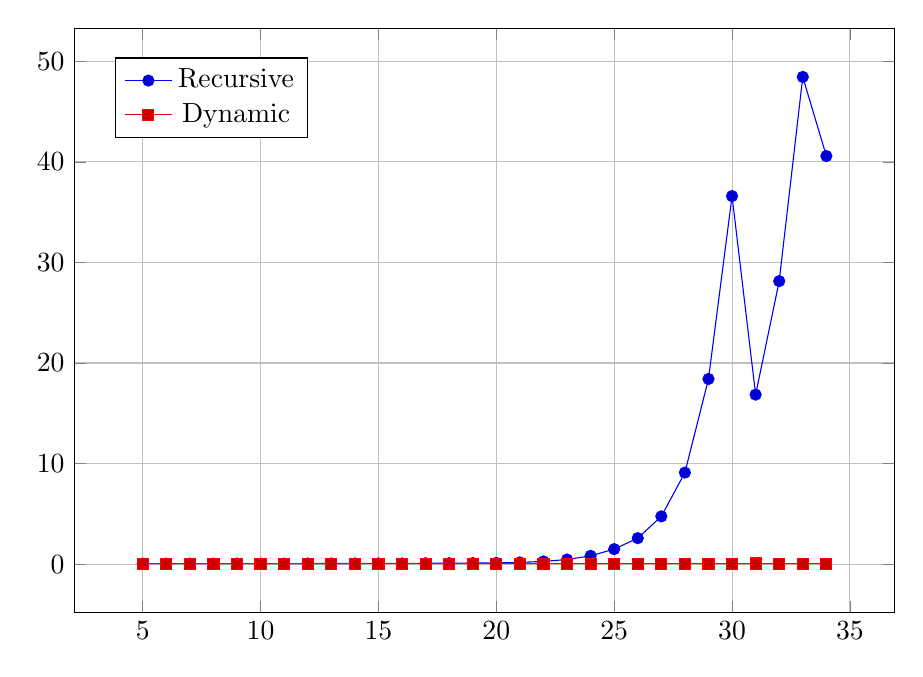
\begin{tikzpicture}
    \begin{axis}[height=9cm, width=12cm, grid=major,legend style={at={(0.05,0.95)},anchor=north west}]
    \addplot coordinates {
(5,0.059)
(6,0.053)
(7,0.056)
(8,0.056)
(9,0.064)
(10,0.055)
(11,0.055)
(12,0.065)
(13,0.068)
(14,0.071)
(15,0.075)
(16,0.075)
(17,0.087)
(18,0.100)
(19,0.110)
(20,0.128)
(21,0.173)
(22,0.274)
(23,0.460)
(24,0.830)
(25,1.497)
(26,2.587)
(27,4.753)
(28,9.104)
(29,18.413)
(30,36.596)
(31,16.855)
(32,28.140)
(33,48.443)
(34,40.577)
    };
    \addlegendentry{Recursive}
        \addplot coordinates {
(5,0.049)
(6,0.051)
(7,0.054)
(8,0.050)
(9,0.056)
(10,0.051)
(11,0.052)
(12,0.051)
(13,0.050)
(14,0.052)
(15,0.050)
(16,0.051)
(17,0.055)
(18,0.050)
(19,0.054)
(20,0.052)
(21,0.050)
(22,0.053)
(23,0.050)
(24,0.057)
(25,0.050)
(26,0.050)
(27,0.052)
(28,0.053)
(29,0.049)
(30,0.051)
(31,0.060)
(32,0.052)
(33,0.057)
(34,0.058)
        };
        \addlegendentry{Dynamic}
    \end{axis}
\end{tikzpicture}
\end{document}
